\chapter{Реализация}
\label{chap:impl}
В этой главе дается подробное описание реализации анализаторов промежуточного представления EO. Раздел \ref{impl:data_structures} описывает общие структуры данных, используемые анализаторами. Разделы \ref{impl:mutualrec} и \ref{impl:unjustified} описывают алгоритмы анализа и их реализации.

\section{Структуры данных}
\label{impl:data_structures}

\subsection{Синтаксическое дерево EO}
Это структура данных, которая используется для моделирования синтаксической структуры EO, которая используется как отправная точка для извлечения более высокоуровневых понятий, таких как класс-объекты, метод-объекты и вызовы методов. Он описывает EO, следуя спецификации синтаксиса из статьи Бугаенко \cite{eolang}, с небольшими отклонениями для учета специфики лежащего в основе уточненного $\varphi$-исчисления, описанного в \cite{kudasov}. 

Для создания синтаксического анализатора от кода EO к синтаксическому дереву EO мы использовали \textbf{cats-parse} \footnote{\url{https://github.com/typelevel/cats-parse}}, монадический синтаксический комбинатор \cite{hill_combinators_1996}, библиотека для Scala.

Синтаксическое дерево EO - это неизменяемая полиморфная структура данных, определяемая \textit{à la carte} \cite{alacarte} \pic{fig:ast}. 
Поскольку дерево неизменяемо, оно может быть изменено только путем построения новой версии, в которой старые части дерева заменяются новыми. Преобразования, которые строят эти новые версии структуры данных, известны как \textit{optics} \cite{optics}. Мы использовали \textit{monocle} \footnote{\url{https://www.optics.dev/Monocle/}} библиотеку для Scala, чтобы упростить генерацию оптик, которые изменяют синтаксическое дерево EO.  

\begin{figure}
    \lstinputlisting[language=Scala]{code/ast.scala}
    \caption{Определения синтаксического дерева EO (сокращенно)}.
    \label{fig:ast}
\end{figure}
\subsection{Объектное дерево}
Дерево объектов является структурой данных, которая фиксирует отношения между объектами в программе EO. Оно является уточнением синтаксического дерева EO, которое содержит элементы программы EO, относящиеся к последующим шагам анализа: классы-объекты, методы-объекты, пункты расширения и вызовы методов. 

Дерево объектов EO также является рекурсивно-определенной полиморфной структурой данных \pic{fig:objtree}. Параметр типа $A$ представляет информацию, которая хранится для каждого объекта в дереве. Эта информация хранится в поле \textit{info} дерева. Поле \textit{nestedObjs} хранит информацию обо всех вложенных классах-объектах. Вложенные объекты - это классы-объекты, которые определяются как атрибуты других объектов класса, подобно вложенным классам в Java. Информация об одном из вложенных объектов может быть доступна по ключу, который имеет тип \textit{Name}. Это имя однозначно идентифицирует объект, так как объект не может содержать два атрибута с одинаковым именем.  

\begin{figure}
    \begin{lstlisting}
        final case class ObjectTree[A](
          info: A,
          nestedObjs: Map[Name, ObjectTree[A]]]
        ) 
    \end{lstlisting}
    \caption{Объектное дерево}
    \label{fig:objtree}
\end{figure}

\subsection{ObjectInfo}

Первый и наиболее общеприменимый тип, который мы используем вместо параметра типа $A$ - это \textit{ObjectInfo} \pic{fig:objinfo}. Этот тип также имеет два параметра типа. Первый, $P$, отвечает за хранение информации о декорированном объекте (или просто родителе). Первый обход может собрать только имя декорированного объекта. 

Второй параметр типа, $M$, - это тип, используемый для хранения информации о каждом из методов. Информация, полученная во время первого обхода синтаксического дерева EO \pic{fig:methodinfo}, может быть обобщена следующим образом:

\begin{itemize}
    \item \textit{selfArgName} - имя свободного атрибута объекта метода, который используется для захвата вызывающего объекта. 
    \item \textit{body} - узел синтаксического дерева EO, который содержит тело метода. 
    \item \textit{depth} - насколько глубоко вложен объект метода в программу EO. Для объектов верхнего уровня этот атрибут равен $0$. Для объектов методов (которые всегда определены в классах-объектах), этот атрибут равен глубине класса-объекта плюс один.  
    \item \textit{calls} - последовательность вызовов метода в определении метода. Тип \textit{Call} хранит всю необходимую информацию для идентификации и обхода всех вызовов в теле метода:
    \begin{itemize}
        \item depth - глубина объекта, в котором находится вызов. Это значение равно глубине метода-объекта + относительная глубина метода-локального объекта, содержащего вызов.
        \item \textit{methodName} - простое имя метода-объекта, в котором находится вызов.
        \item \textit{callSite} - оптика \cite{optics}, которая извлекает местоположение метода-локального объекта, где находится вызов. 
        \item \textit{callLocation} - оптика \cite{optics}, которая извлекает местоположение узла синтаксического дерева EO, который определяет вызов метода. 
        \item \textit{args} - узлы синтаксического дерева EO, которые соответствуют аргументам вызова, включая аргумент \textbf{self}.  
    \end{itemize}  
\end{itemize}

\begin{figure}
    \begin{lstlisting}[language=Scala]
      final case class ObjectInfo[P, M](
        name: Name,
        fqn: FQName,
        depth: Int,
        parentInfo: Option[P],
        методы: Map[Name, M],
      )
    \end{lstlisting}
    \caption{ObjectInfo}
    \label{fig:objinfo}
\end{figure}

\begin{figure}
    \begin{lstlisting}[language=Scala]
      final case class MethodInfo(
          selfArgName: String,
          вызовы: Vector[Call],
          тело: EOObj[EOExprOnly],
          глубина: Int,
      )
          
      final case class Call(
        глубина: BigInt,
        methodName: String,
        callSite: PathToCallSite,
        callLocation: PathToCall,
        args: NonEmptyVector[EOBnd[EOExprOnly]]
      )
    \end{lstlisting}
    \caption{МетодИнфо и вызов}
    \label{fig:methodinfo}
\end{figure}

\subsection{Частичное дерево объектов}
\textit{ObjectInfo}, где $P$ - имя родительского объекта, а $M$ - \textit{MethodInfo}, можно назвать \textit{частичным деревом объектов}:
\begin{lstlisting}
    тип PartialObjectTree = ObjectTree[
        ObjectInfo[ParentName, MethodInfo]
    ]

\end{lstlisting}

\subsection{Полное дерево объектов}
\label{impl:complete_object_tree}
Так называемое \textit{полное дерево объектов} определяется как следующий псевдоним типа:
\begin{lstlisting}[language=Scala]
  type CompleteObjectTree =
    ObjectTree[
      ObjectInfo[
        LinkToParent,
        MethodInfo
      ]
    ]
\end{lstlisting}
Единственное, что отличает его от \textit{частичное дерево объектов}, это то, что имя родителя заменяется специальным типом \textit{LinkToParent}. Этот тип также является оптическим \cite{optics} и по сути является функцией типа:
\begin{lstlisting}[language=Scala].
    val linkToParent: 
      CompleteObjectTree => CompleteObjectTree
\end{lstlisting}
Берется все дерево объектов программы и возвращается объект, который представляет собой декорированный объект объекта, на который находится ссылка.



\section{Нахождение непредвиденной взаимной рекурсии}
\label{impl:mutualrec}

\subsection{Предлагаемое решение}
\label{impl:mutualrec_algo}
Решение проблемы заключается в обнаружении циклов в графах вызовов всех объектов. Для каждого класса-объекта в программе сделайте следующее:
\begin{enumerate}
    \item Определить декорированный класс-объект, все методы, и для каждого метода в классе определить все методы, которые он вызывает. Если вызываемый метод существует в классе-объекте, пометьте его как \textit{решенный}. В противном случае, пометьте его как \textit{частично решенный}. Набор отображений между методами класса и методами, которые каждый из методов вызывает, считается \textit{частичным графом вызовов} объекта.
    \item После этого дерево снова обходится, чтобы преобразовать все частично разрешенные вызовы в полностью разрешенные. Для этого нужно вычислить \textit{полный граф вызовов} объекта, который содержит методы из самого объекта, а также методы из декорированного объекта. Это делается путем \textit{расширения} частичного call-графа декорированного объекта с частичным call-графом декорирующих объектов. Здесь и далее мы используем термины \textbf{ребенок} и \textbf{родитель} для обозначения декорирующего объекта и декорируемого объекта соответственно. Процедура расширения определяется следующим образом:
          \begin{enumerate}
              \item если метод присутствует в родительском колл-графе, но отсутствует в дочернем колл-графе, он оставляется как есть.
              \item если метод присутствует в дочернем колл-графе, но не существует в родительском колл-графе, он добавляется в родительский колл-граф.
              \item если метод присутствует и в дочернем, и в родительском колл-графе, все вхождения метода в родительском колл-графе заменяются дочерней версией метода.
          \end{enumerate}
    \item После того, как граф вызовов объекта разрешен, выполните поиск в глубину по первому слову \cite{dfs}, чтобы найти циклы в полном графе вызовов. После того, как все циклы будут найдены, исключите циклы, которые содержат только методы одного и того же объекта.
\end{enumerate}

\subsection{Реализация}
Первый шаг алгоритма в \ref{impl:mutualrec_algo} заключается в преобразовании кода EO в \textit{полное дерево объектов} (раздел \ref{impl:complete_object_tree}). Затем объектное дерево преобразуется в вариацию объектного дерева, где все вызовы разрешены. Эта вариация называется \textit{ObjectTreeWithResolvedCallgraphs} \pic{fig:mutualrec_program}. Для каждого объекта хранится только его полностью разрешенный граф вызовов. Последний шаг обходит дерево и собирает все циклы в список специальных объектов типа \textit{CallChain}. Этот объект представляет собой последовательность полностью вычисленных имен методов, которые при вызове никогда не завершаются. Наконец, каждая из таких цепочек вызовов представляется пользователю в виде человекочитаемых строк. 

\begin{figure}
    \begin{lstlisting}[language=Scala]
        type ResolvedCallGraph = 
          Map[Methodname, Set[MethodName]]
        type ObjectTreeWithResolvedCallgraphs =
          ObjectTree[ResolvedCallGraph]
    \end{lstlisting}
    \caption{\textit{ObjectTreeWithResolvedCallgraphs}}.
    \label{fig:mutualrec_program}
\end{figure}

\section{Нахождение необоснованного предположения в подклассах}
\label{impl:unjustified}

\subsection{Предлагаемое решение}
\label{impl:unjustified_algo}
Мы предлагаем следующий подход для обнаружения методов, в которых инлайнинг вызовов может привести к ломающим изменениям в подклассах:
\begin{enumerate}
    \item Создается \textit{изначальное} представление программы. Это представление представляет собой древовидную структуру данных, которая сохраняет отношения вложенности между объектами. Так, объекты, которые содержат другие объекты, являются корнями соответствующих поддеревьев, в то время как объекты-контейнеры являются поддеревьями или листьями.
    \item Мы создаем \textit{ревизию} исходного представления программы, где все вызовы методов инлайнированы.
    В обеих версиях для каждого класса-объекта, для каждого метода в классе-объекте, определяется набор \textit{свойств}.  Эти свойства можно рассматривать как неявный контракт \cite{meyer} каждого метода. В дополнение к неявным свойствам, учитываются и явные свойства, которые приходят в виде \textit{assert} утверждений в исходном коде. Для того чтобы определить свойства метода, выполняется частичная интерпретация его тела. Интерпретация ограничивается основными числовыми операциями, числовыми и булевыми значениями и вызовами методов. Более подробно правила вывода описаны на рис. \ref{fig:property_inference}.
    \item После того, как все свойства выведены, следующий предикат должен быть истинным как для первоначальной, так и для измененной версии:
          \begin{align}
              P_{init} \implies P_{rev}
              \label{fig:implication}
          \end{align}
          Если это не выполняется для какого-то класса-объекта, это означает, что пересмотр одного из его суперклассов вносит разрывное изменение, которое ослабляет предусловие некоторых его методов.
\end{enumerate}

\begin{figure}
  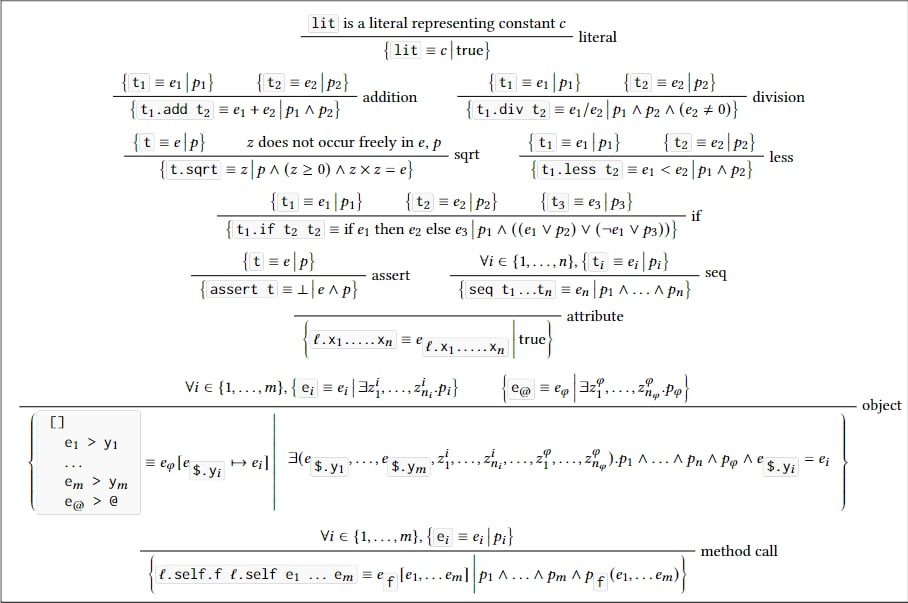
\includegraphics[width=\textwidth]{figs/properties}
  \caption{Правила вывода свойств при обнаружении необоснованного предположения в подклассе.}
  \label{fig:property_inference}
\end{figure}


\subsection{Реализация}
Аналогично алгоритму обнаружения взаимной рекурсии, древовидное представление начальной ревизии программы EO осуществляется путем преобразования ее исходного кода в \textit{полное дерево объектов} (раздел \ref{impl:complete_object_tree}). Однако для того, чтобы произвести ревизию исходной программы, нам потребовалось реализовать процедуру инлайнинга для синтаксического дерева EO. Эта процедура может быть представлена следующим образом:
\begin{enumerate}
  \item Определить все вызовы методов. Это уже сделано во время построения полного дерева объектов.
  \item Заменить каждый вызов метода в теле метода значением его $\varphi$-атрибута (символ @ в eo).
  \item Если метод-объект, который декорируется, содержит атрибуты, отличные от $\varphi$, то:
  \begin{enumerate}
    \item собирает эти атрибуты в отдельный объект под названием \textit{local\_attrs}. Если атрибут с таким именем уже существует в объекте, в который вставляется вызов, разрешите коллизию, добавив суффикс к вновь созданному объекту. 
    \item Добавить этот объект в качестве локального атрибута к методу-объекту, в котором находится вызов. 
    \item Перенаправить ссылки на локальные атрибуты внутри атрибута $\varphi$ метода, который инлайнится, на их соответствующие атрибуты в объекте \textit{local\_attrs}.
  \end{enumerate}

  \item После того, как пересмотр исходного кода EO получен, исходное дерево объектов и пересмотренное дерево объектов сшиваются вместе в отдельный экземпляр дерева объектов \pic{fig:zipwithinlined}.

  \item Теперь, когда у нас есть вся необходимая информация о первоначальной и пересмотренной версиях, нам нужно вывести их свойства \pic{fig:property_inference}. Эти свойства закодированы в виде программ SMTLIB2 \cite{smtlib}. Мы используем \textbf{scala-smtlib} \footnote{\url{https://github.com/regb/scala-smtlib}} библиотеку для программного построения SMTLIB2-совместимых программ. Эти программы хранятся во вспомогательной структуре данных \ref{fig:property_structure}. Эта структура имеет следующие поля.
  \item Когда эта структура построена как для первоначальной, так и для пересмотренной версии, строится оператор импликации, соответствующий формуле \pic{fig:implication} и передается бэкенду SMT-решателя. Бэкенд, который мы используем в данной диссертации, называется Princess \cite{princess}.
  \item Если решатель находит данное предложение удовлетворяющим, то ошибки нет, и ревизия считается безопасной. В противном случае ревизия считается небезопасной и о ней сообщается пользователю. 
\end{enumerate}

\begin{figure}
    \begin{lstlisting}[language=Scala]
      final case class Info(
        forall: List[SortedVar],
        exists: List[SortedVar],
        value: Term,
        properties: Term
      )
    \end{lstlisting}
    \caption{Структура данных для хранения производных свойств.}
    \label{fig:property_structure}
    \end{figure}
    
    \begin{figure}
    \begin{lstlisting}[language=Scala]
      final case class MethodInfoForAnalysis(
        selfArgName: String,
        тело: EOObj[EOExprOnly],
        глубина: Int
      )
    
      final case class ObjectInfoForAnalysis[P, M](
        methods: Map[EONamedBnd, M],
        parentInfo: Option[P],
        name: Name,
        indirectMethods: Map[
          Name, 
          MethodInfoForAnalysis
        ],
        allMethods: Map[
          Name, 
          MethodInfoForAnalysis
        ]
      )
    
      type AnalysisInfo = ObjectInfoForAnalysis[
        LinkToParent,
        MethodInfo
      ]
      type InitialAndRevised = ObjectTree[
          (AnalysisInfo, AnalysisInfo)
        ]
    \end{lstlisting}
    \caption{Дерево объектов, используемое в анализе необоснованных предположений, которое содержит пересмотренную версию объекта вместе с первоначальной версией.}
    \label{fig:zipwithinlined}
    \end{figure}
    